\chapter{Mechanical Model of the Heart}
\label{sec:model}

\section{Introduction}
In this chapter we describe the anatomical structure of the human heart and describe how we translate that information to build a simple mechanical model of the heart. This mechanical model is used to constrain the problem of cardiac motion estimation, as shall be explained in detail in Section \ref{chap:inverse}. The heart is a complicated system, with an electro-mechanical system responsible for the activation and contraction of the heart muscles. Modeling of cardiac anatomy, electrophysiology and mechanics is an active research field. A comprehensive review of the field can be found in \cite {sachse04}. Muscle fiber orientations need to be considered while modeling cardiac electro-mechanics. The diffusion properties of the muscle fibers play an important role in the propagation of cardiac activation current. Similarly the force generated by the muscles is along the fiber direction. Therefore knowledge of the diffusion tensor or at least the fiber orientations is very important for modeling purposes, especially if the models are patient specific. It is not possible to obtain diffusion tensor images in vivo currently, and as a result most modeling approaches use synthetic data for the fiber orientations. These models for fiber orientations are very simple and capture only the basic trends in the orientation. Since our goal is to estimate the motion of the heart, we ignore the electrical stimulation that activates the heart muscles and develops the forces in the myo-fibers. Instead we solve for the forces directly, and only model the mechanical aspects of the heart. For this we solve a linear elasticity equation at all the fibers. The model parameters are the fiber orientations, and the material properties. We first describe how these parameters are obtained, followed by the governing equations for the model.

\section{Anatomical Structure of the Heart}
Modeling of cardiac anatomy, electrophysiology, and mechanics is very important for understanding the complicated interactions that take place between different anatomical structures. This knowledge helps us to understand the mechanisms of heart failure, and can help devise ways to prevent and cure such pathologies. A large number of cardiac pathologies occur because of problems with the electro-mechanical system within the heart. Consequently, a lot of active research is being carried out in this field.  A comprehensive review of the field can be found in \cite{mackerle2005fem, sachse04}. 


The walls of the heart are composed of cardiac muscle, called myocardium. It consists of four compartments: the right and left atria and ventricles. The heart is oriented so that the anterior aspect is the right ventricle while the posterior aspect shows the left atrium. The left ventricular free wall and the septum are much thicker than the right ventricular wall. This is logical since the left ventricle pumps blood to the systemic circulation, where the pressure is considerably higher than for the pulmonary circulation, which arises from right ventricular outflow. Since a muscle fiber can contract only in one direction, the heart structure is complex, to succeed at pumping the blood. Anatomically, to achieve this, the muscle walls of the ventricles and the atria are composed of a single helically folded muscular structure as can be seen in Figure \ref{grays_1}. The cardiac muscle fibers are divided into four groups \cite{gray18}: Two groups of fibers wind around the outside of both ventricles. Beneath these fibers a third group winds around both ventricles. Beneath these fibers a fourth group winds only around the left ventricle. 

\begin{figure}[!hbtp]
\begin{center}
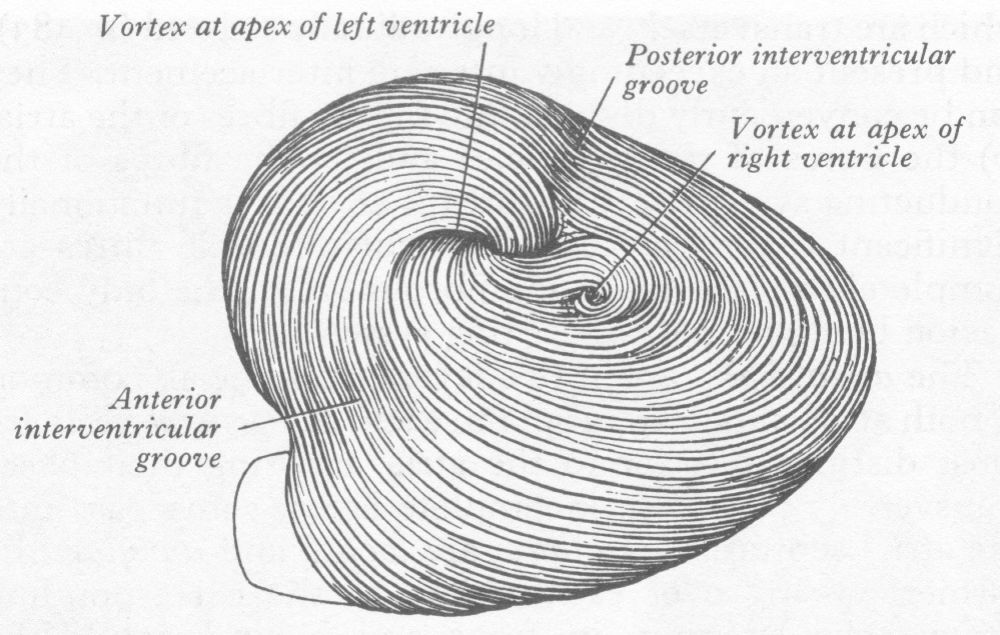
\includegraphics[width=0.4\textwidth]{images/grays_3}
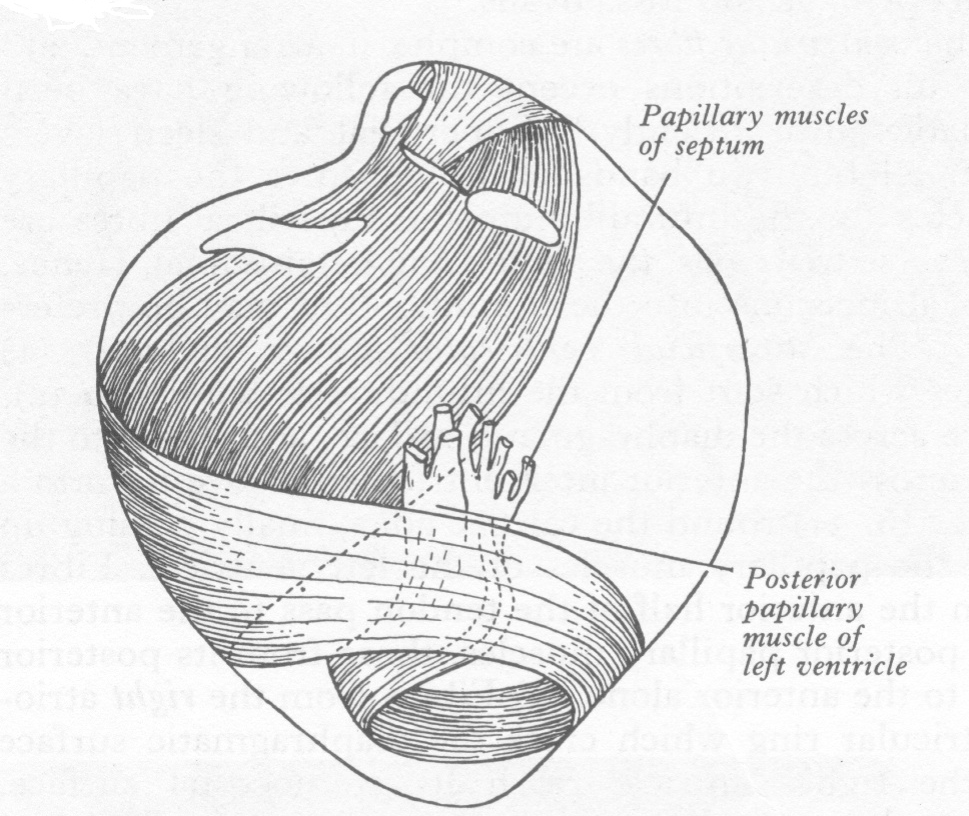
\includegraphics[width=0.34\textwidth]{images/grays_2} 
\caption{\em \small Fiber orientations in the Human Heart showing the helical structure of the muscles (from \cite{gray18})}
\label{grays_1}
\end{center}  
\end{figure} 

\section{Mechanical Modeling}

\[
	\rho \ddot{\bf u} - \mu\Delta{\bf u} + (\lambda+\mu)\nabla {\bf div~} {\bf u} = {\bf f}R({\bf u})\vec{\eta_0}
	\]	

We model the heart as a linear elastic solid occupying a bounded region $\omega$, with Dirichlet boundary conditions. Its displacement is described by 

\begin{equation}
\nabla \cdot \left[\lambda({\bf x})\left(\div \cdot {\bf U} \right) {\bf I} + \mu({\bf x})  \left( \div {\bf U} + (\div {\bf U} )^T \right) \right] + {\bf f}R({\bf U})\bN_0 = 0  \mbox{~~~~in~} \omega \mbox{,~~~~} {\bf U}  = {\bf g} \mbox{~~~~on~} \gamma.
\label{e-linear}
\end{equation}

Here ${\bf u}$ is the displacement field, and $\lambda({\bf x})$ and $\mu({\bf x})$ are the Lam\'{e} parameters which are related to the Young's Modulus $E({\bf x})$ and Poisson's ratio $\nu({\bf x})$. $\bR(\bU)$ is the rotational component of the local displacement field, by which the fiber orientation $\bN_0$ must be rotated. To solve (\ref{e-linear}) we embed $\omega$ in a regular domain $\Omega$. We use trilinear finite elements to discretize (\ref{e-linear}), and piecewise constant functions for $\lambda,\nu$.  The Poisson ratio $\nu({\bf x})$ varies between $0$ for a fully compressible material to $0.5$ for a fully incompressible material. When considering soft tissue deformations, the value of the Poisson ratio given for many tissue classes borders on the limit of incompressibility\footnote{As $\nu$ approaches 0.5, commonly used displacement-based finite element implementations suffer from the so-called locking effect.  We use underintegration for the $\nabla \cdot {\bf u}$ term in (\ref{e-linear}); see \cite{Hughes87} for details.}. Gladilin~\cite{Gladilin2003} studies the sensitivity of the Poisson ratio on the displacement field obtained via an incompressible formulation and a compressible formulation. The results indicate that Poisson ratio does not affect the solution significantly.

\subsection{Linear Elastodynamics}

We assume that the MR image occupies the region $\Omega \in \mathbb{R}^3$ in its reference state (end-diastole) at time $t=0$. The boundary $\Gamma=\partial\Omega$ has the outward unit normal given by $\bn$, the displacement vector is represented by $\bu$, and the velocity by $\bv$. The myocardium is assumed to be made of an elastic material and is subject to body force $\force$ per unit volume.

The strong form of the equations of linear elastodynamics are written as:
\begin{eqnarray}
\rho\dudtsq &=& \div\cdot\stress + \force \qquad \mbox{in} ~\Omega\times]0,T[, \\
\stress \bn &=& 0, \qquad\qquad~~~~ \mbox{in} ~\Gamma\times]0,T[, \nonumber\\
\bu(t=0) &=& \bu_0, \qquad\qquad~~ \mbox{in} ~\Omega \nonumber\\
\dot{\bu}(t=0) &=& \bv_0, \qquad\qquad~~ \mbox{in} ~\Omega \nonumber
\end{eqnarray}
where $\bu_0$ is the initial displacement, $\bv_0$ is the initial velocity, $\stress$ is the stress tensor and $\div\cdot\stress$ denotes the divergence of $\stress$. Assuming that the material is isotropic and homogeneous, one may express the stress tensor as
\begin{equation}
\label{eq:stressstrain}
\stress = \lambda~\mbox{tr}~\strain\bI + 2\mu\strain,
\end{equation}
in terms of the Lam\'{e} constants $\lambda$ and $\mu$, the identity tensor $\bI$, and the infinitesimal strain tensor $\strain$. The strain is defined as
\begin{equation}
\label{eq:strain}
\strain := \frac{1}{2}\left[ \gradu + \gradut \right] := \div_s\bu~,
\end{equation} 
where $\gradu$ is the gradient operator expessed in Cartesian component form as
\[
[\gradu] = \left[ \begin{array}{c}u_1\\u_2\\u_3\end{array}\right] 
\left[\begin{array}{ccc} \dfrac{\partial}{\partial x} & \dfrac{\partial}{\partial y} & \dfrac{\partial}{\partial z} \end{array}\right] =
\left[
\begin{array}{ccc} 
u_{1,1} & u_{1,2} & u_{1,3} \\
u_{2,1} & u_{2,2} & u_{2,3} \\
u_{3,1} & u_{3,2} & u_{3,3}
\end{array}
\right] ~.
\]
Using equation (\ref{eq:strain}), the components of the strain tensor are
\[
[\strain] = \left[
\begin{array}{ccc} 
u_{1,1} & \frac{1}{2}(u_{1,2}+u_{2,1}) & \frac{1}{2}(u_{1,3}+u_{3,1}) \\
\frac{1}{2}(u_{1,2}+u_{2,1}) & u_{2,2} & \frac{1}{2}(u_{2,3}+u_{3,2}) \\
\frac{1}{2}(u_{1,3}+u_{3,1}) & \frac{1}{2}(u_{2,3}+u_{3,2}) & u_{3,3}
\end{array}
\right] ~.
\]

%% Variational formulation
Let $\bw$ denote the variations, and $\bw \in \mathcal{V}$ the variation space.
Then the weak form can be written as
\begin{equation}
\int_{\Omega} \bw\cdot(\rho\dudtsq-\div\cdot\stress -\force)~d\Omega + \int_{\Gamma} \bw\cdot\stress\bn~d\Gamma = 0.
\end{equation}
Using the Einsteinian summation convention, we can write it as,

\begin{eqnarray}
  0 & = & \int_{\Omega} w_i ( \rho u_{i, t t} - \sigma_{i j, j} - f_i )~d\Omega + \int_{\Gamma} w_i \sigma_{ij} n_j~d \Gamma \nonumber\\
	& = & \int_{\Omega} w_i \rho_i u_{i, t t}~d\Omega - 	
	\left(	\int_{\Omega} w_i\sigma_{ij,j}~d\Omega \right) -
  \int_{\Omega} w_i f_i~d\Omega + \int_{\Gamma} w_i \sigma_{ij} n_j~d\Gamma \nonumber\\
  & = & \int_{\Omega} w_i \rho_i u_{i, t t}~d\Omega - 	
	\left(	\int_{\Omega} (w_i\sigma_{ij})_{,j}~d\Omega - \int_{\Omega} w_{i,j}\sigma_{ij}~d\Omega \right) -
  \int_{\Omega} w_i f_i~d\Omega + \int_{\Gamma} w_i \sigma_{ij} n_j~d\Gamma \nonumber\\
	& = & \int_{\Omega} w_i \rho_i u_{i, t t}~d\Omega - 	
	\left( \int_{\Gamma} w_i \sigma_{ij} n_j~d\Gamma - \int_{\Omega} w_{i, j}\sigma_{ij}~d\Omega \right) -
  \int_{\Omega} w_i f_i~d\Omega + \int_{\Gamma} w_i \sigma_{ij} n_j~d\Gamma \nonumber\\
  & = & \int_{\Omega} w_i \rho_i u_{i, t t}~d\Omega + \int_{\Omega} w_{( i, j )} \sigma_{ij}~d\Omega - \int_{\Omega} w_i f_i~d\Omega,
\end{eqnarray}
where use is made of integration by parts and the divergence theorem. It follows that,
\begin{equation}
\label{eq:weakForm}
\int_{\Omega} \bw\cdot\rho\ddot{\bu} ~d\Omega - \int_{\Omega}\div_s\bw:\stress ~d\Omega = \int_{\Omega} \bw\cdot\force ~d\Omega ~,
\end{equation}
where $\div_s\bw:\stress$ denotes the contraction of the tensors $\div_s\bw$ and $\stress$, expressed in component form as $\div_s\bw:\stress=w_{i,j}\sigma_{ij}$.

Equation (\ref{eq:weakForm}) motivates us to define the following bilinear forms:
\begin{eqnarray}
  a (\bw,\bu) & = & -\int_{\Omega}\div_s\bw:\stress ~d\Omega, \label{eq:bilinear} \\ %= \int_{\Omega} w_{( i, j )} \sigma_{ij}~d\Omega\\
  (\bw,\force) & = & \int_{\Omega} \bw\cdot\force ~d\Omega, ~\mbox{and}~ \\ %= \int_{\Omega} w_i f_i~d\Omega \nonumber\\
  (\bw, \rho \ddot{\bu} ) & = & \int_{\Omega} \bw\cdot\rho\ddot{\bu} ~d\Omega. % = \int_{\Omega} w_i \rho u_{i, t t} d \Omega \nonumber
\end{eqnarray}
The corresponding weak formulation can be written as:

Given $\force, \bu_0 \tmop{and} \bv_0$, find $\bu( t ) \in \mathcal{S}_t, t \in [ 0, T ]$,
such that for all $\bw \in \mathcal{V}$, such that 
\begin{eqnarray}
  (\bw, \rho \ddot{\bu} ) + a (\bw,\bu) &
  = & (\bw,\force), \\
  (\bw, \rho \bu( 0 ) ) & = & (\bw, \rho \bu_0 ), \nonumber\\
  (\bw, \rho \dot{\bu} ( 0 ) ) & = & (\bw, \rho \tmmathbf{v}_0 ) \nonumber.
\end{eqnarray}

In order to simply the expressions, we express the components of tensorial quantities such as $\div_s\bw$ and $\stress$ in vector form. In particular we define the strain vector as,  

\[ 
	\strain(\bu) = 
	\left\{ \begin{array}{c}
	\epsilon_{11} \\ \epsilon_{22} \\ \epsilon_{33} \\
	2\epsilon_{12} \\ 2\epsilon_{23} \\ 2\epsilon_{31}
	\end{array} \right\}  =
	\left\{ \begin{array}{c}
     u_{1, 1}\\
     u_{2, 2}\\
     u_{3, 3}\\
     u_{2, 3} + u_{3, 2}\\
     u_{1, 3} + u_{3, 1}\\
     u_{1, 2} + u_{2, 1}
   \end{array} \right\} 
\]

Likewise, the stress tensor can be written in vector form as,

\[
\stress = \left\{ \begin{array}{c}
	\sigma_{11} \\ \sigma_{22} \\ \sigma_{33} \\
	\sigma_{12} \\ \sigma_{23} \\ \sigma_{31} \end{array} \right\} 
\]

The stress-strain law (\ref{eq:stressstrain}) can be written using the vector convention as
\begin{equation}
\label{ref:stressstrainMat}
[\stress] = [\bD][\strain],
\end{equation} 

where $[\bD]$ is a ($6\times6$) elasticity matrix such that
\begin{equation}
  \bD= \left[ \begin{array}{cccccc}
    \lambda + 2 \mu & \lambda & \lambda & 0 & 0 & 0\\
    \lambda & \lambda + 2 \mu & \lambda & 0 & 0 & 0\\
    \lambda & \lambda & \lambda + 2 \mu & 0 & 0 & 0\\
    0 & 0 & 0 & \mu & 0 & 0\\
    0 & 0 & 0 & 0 & \mu & 0\\
    0 & 0 & 0 & 0 & 0 & \mu
  \end{array} \right]
\end{equation}

Since the matrix $[\bD]$ is always symmetric, it follows that the integrand of the bilinear form in (\ref{eq:bilinear}) can be written with the aid of (\ref{ref:stressstrainMat}) as

\[
\div_s\bw:\stress = [\strain(\bw)][\bD][\strain(\bu)] := \strain(\bw)\cdot\bD\strain(\bu) ,
\]
which shows that the bilinear form in (\ref{eq:bilinear}) in indeed symmetric. 

\subsection{Semidiscrete Galerkin formulation of elastodynamics}

Given $\force, \bu_0, \tmop{and} \dot{\bu_0}$, find $\bu^h =\bv^h
+\tmmathbf{g}^h,\bu^h ( t ) \in \mathcal{S}_t^h$, such that for all
$\bw^h \in \mathcal{V}^h$,
\begin{eqnarray}
  (\bw^h, \rho \ddot{\tmmathbf{v}}^h ) + a
  (\bw^h,\tmmathbf{v}^h ) & = & (\bw^h, f ) 
- (\bw^h, \rho \ddot{\tmmathbf{g}}^h ) - a (\bw^h,\tmmathbf{g}^h ) \nonumber\\
  (\bw^h, \rho \tmmathbf{v}^h ( 0 ) ) & = & (\bw^h, \rho
  \bu_0 ) - (\bw^h, \rho \tmmathbf{g}^h ( 0 ) ) \nonumber\\
  (\bw^h, \rho \dot{\tmmathbf{v}}^h ( 0 ) ) & = & (\bw^h,
  \rho \dot{\bu}_0 ) - (\bw^h, \rho \dot{\tmmathbf{g}}^h ( 0
  ) ) 
\end{eqnarray}
The representations of $\bw^h,\tmmathbf{v}^h \tmop{and}
\tmmathbf{g}^h$ are given by
\begin{eqnarray}
  \bw^h (\tmmathbf{x}, t ) = w_i^h (\tmmathbf{x}, t )\tmmathbf{e}_i &
  = & \sum_{A \in \eta - \eta_{q_i}} N_A (\tmmathbf{x}) c_{i A} ( t
  )\tmmathbf{e}_i \nonumber\\
  \tmmathbf{v}^h (\tmmathbf{x}, t ) = v_i^h (\tmmathbf{x}, t )\tmmathbf{e}_i &
  = & \sum_{A \in \eta - \eta_{g_i}} N_A (\tmmathbf{x}) d_{i A} ( t
  )\tmmathbf{e}_i \nonumber\\
  \tmmathbf{g}^h (\tmmathbf{x}, t ) = g_i^h (\tmmathbf{x}, t )\tmmathbf{e}_i &
  = & \sum_{A \in \eta_{g_i}} N_A (\tmmathbf{x}) g_{i A} ( t )\tmmathbf{e}_i 
\end{eqnarray}
Substituting (14) into (13) we get, (ignoring $\tmmathbf{e}_i, \tmop{and}
\tmmathbf{e}_j$ for clarity,

\begin{eqnarray*}
& & \left( \sum_{A \in \eta_{\tmop{int}}} N_A (\tmmathbf{x}) c_{i A} ( t ),
   \sum_{B \in \eta_{\tmop{int}}} N_B (\tmmathbf{x}) \rho \ddot{d_{}}_{j B} (
   t ) \right) + a \left( \sum_{A \in \eta_{\tmop{int}}} N_A (\tmmathbf{x})
   c_{i A} ( t ), \sum_{B \in \eta_{\tmop{int}}} N_B (\tmmathbf{x}) d_{i B} (
   t ) \right) \\
&=& \left( \sum_{A \in \eta_{\tmop{int}}} N_A (\tmmathbf{x}) c_{i
   A} ( t ),\force \right) + \left( \sum_{A \in \eta_{\tmop{int}}} N_A
   (\tmmathbf{x}) c_{i A} ( t ),\mathfrak{h} \right)_{\Gamma} -   
   \left( \sum_{A \in \eta_{\tmop{int}}} N_A (\tmmathbf{x}) c_{i A} ( t ),
   \sum_{B \in \eta_{q_i}} N_B \rho \ddot{g}_{i B} ( t ) \right) \\
&-& a\left(  \sum_{A \in \eta_{\tmop{int}}} N_A (\tmmathbf{x}) c_{i A} ( t ), \sum_{B
   \in \eta_{q_i}} N_B g_{i B} ( t ) \right) 
\end{eqnarray*}

This gives us a set of $3 \eta_{\tmop{int}} = 3 ( \eta - \eta_{q_i} )$
equations, where $\eta$ is the total number of nodes,
\begin{eqnarray*}
& & \sum^{n_{\tmop{dof}}}_{j = 1} \sum_{B \in \eta_{\tmop{int}}} ( N_A
  \tmmathbf{e}_i, N_B \tmmathbf{e}_j ) \rho \ddot{d}_{j B} ( t ) + \sum_{j =
  1}^{n_{\tmop{dof}}} \sum_{B \in \eta_{\tmop{int}}} a ( N_A \tmmathbf{e}_i,
  N_B \tmmathbf{e}_j ) d_{j B} ( t ) \\
&=& ( N_A \tmmathbf{e}_i,\force) + ( N_A \tmmathbf{e}_j,\mathfrak{h})_{\Gamma}  - \sum^{n_{\tmop{dof}}}_{j = 1}
  \sum_{B \in \eta_{q_j}} ( N_A \tmmathbf{e}_i, N_B \tmmathbf{e}_j ) \rho
  \ddot{g}_{j B} ( t ) - \sum_{B \in \eta_{q_j}} a ( N_A \tmmathbf{e}_i, N_B
  \tmmathbf{e}_j ) g_{j B} ( t )
\end{eqnarray*}


For the case of homogeneous dirichlet boundary conditions, $\tmmathbf{g}= 0,
\tmop{and} \eta_{q_i} = 0$, therefore (10) reduces to a set of $3 \eta$
equations in $3 \eta$ unknowns,
\begin{equation}
  \sum^{n_{\tmop{dof}}}_{j = 1} \sum_{B \in \eta} ( N_A \tmmathbf{e}_i, N_B
  \tmmathbf{e}_j ) \rho \ddot{d}_{j B} ( t ) + \sum^{n_{\tmop{dof}}}_{j = 1}
  \sum_{B \in \eta} a ( N_A \tmmathbf{e}_i, N_B \tmmathbf{e}_j ) d_{j B} ( t )
  = ( N_A \tmmathbf{e}_i,\force) + ( N_A
  \tmmathbf{e}_i,\mathfrak{h})_{\Gamma}
\end{equation}
In order to derive the mass matrix, the global stiffness matrix and the force
vector, we need to specify the global ordering of equations. This shall be
explained in detail later, for now we assume we have a function
{\tmstrong{id(i,A)}} that takes the degree of freedom and the global node
number as input and returns the global equation number. Using this we can
write the {\tmstrong{matrix problem}} as:

%\begin{tabular}{|c|}
%  \hline \\
%  \begin{eqnarray}
%    \tmmathbf{M} \ddot{\tmmathbf{d}} +\tmmathbf{K} \tmmathbf{d} & = &
%    \force \nonumber\\
%    \tmmathbf{d}( 0 ) & = & \tmmathbf{d}_0 \nonumber\\
%    \dot{\tmmathbf{d}} ( 0 ) & = & \dot{\tmmathbf{d}}_0 
%  \end{eqnarray}
%  \hline
%\end{tabular}

where the mass matrix,
\[ \tmmathbf{M}= \bigwedge_{e = 1}^{n_{\tmop{el}}} (\tmmathbf{m}^e ) \]
here, $\bigwedge$is the matrix assembly operator, and the elemental mass
matrix, $\tmmathbf{m}^e$ is given in terms of nodal submatrices as,
\begin{eqnarray}
  \tmmathbf{m}^e & = & \left[ m_{p q}^e \right] \nonumber\\
  m_{p q}^e & = & \delta_{i j} \int_{\Omega_e} N_a \rho N_b d \Omega 
\end{eqnarray}
\begin{notation}
  In all these definitions, $n_{\tmop{en}}$ is the number of element nodes,
  which for the trilinear hexahedral element is 8; $n_{\tmop{ed}}$ is the
  number of element degrees of freedom per node, which is 3 in our case. Also
  $n_{\tmop{ee}}$ stands for the number of element equations, which is
  $n_{\tmop{ed}} n_{\tmop{en}}$.
\end{notation}

\begin{notation}
  For the elemental mass matrix, $1 \leqslant p, q \leqslant n_{\tmop{ee}} =
  n_{\tmop{ed}} n_{\tmop{en}}$. Therefore in our case the elemental mass
  matrix shall be $24 \times 24$. For the nodal submatrices, indices  $p =
  n_{\tmop{ed}} ( a - 1 ) + i$, and $q = n_{\tmop{ed}} ( b - 1 ) + j$. 
\end{notation}

Similarly, the stiffness matrix can be written as,
\begin{eqnarray}
  \tmmathbf{K} & = & \bigwedge_{e = 1}^{n_{\tmop{el}}} (\tmmathbf{k}^e )
  \nonumber\\
  \tmmathbf{k}^e & = & \left[ k_{p q}^e \right] \nonumber\\
  k_{p q}^e & = & \tmmathbf{e}_i^T \int_{\Omega_e} \tmmathbf{B}_a^T
  \tmmathbf{D} \tmmathbf{B}_a d \Omega \tmmathbf{e}_j 
\end{eqnarray}
where the matrices $\tmmathbf{D}$ was defined earlier (7) and $\tmmathbf{B}_a$
is given by,
\begin{eqnarray*}
  \tmmathbf{B}_a & = & \left[ \begin{array}{ccc}
    N_{a, x} & 0 & 0\\
    0 & N_{a, y} & 0\\
    0 & 0 & N_{a, z}\\
    0 & N_{a, z} & N_{a, y}\\
    N_{a, z} & 0 & N_{a, x}\\
    N_{a, y} & N_{a, x} & 0
  \end{array} \right]
\end{eqnarray*}
We can now proceed to write the right hand side of our equation, i.e., the
force vector. This can be written as,
\begin{eqnarray}
  \force( t ) & = & \force_{\tmop{nodal}} ( t ) +
  \bigwedge_{e = 1}^{n_{\tmop{el}}} (\force^e ( t ) ) \nonumber\\
  \force^e & = & \{ f_p^e \} \nonumber\\
  f_p^e & = & \int_{\Omega_e} N_a f_i d \Omega +
  \int_{\Gamma_{\mathfrak{h}_i}} N_a \mathfrak{h}_i d \Gamma 
\end{eqnarray}
Also, we get the expressions for the initial conditions as,
\begin{eqnarray*}
  \tmmathbf{d}_0 & = & \tmmathbf{M}^{- 1} \bigwedge_{e =
  1}^{n_{\tmop{el}}} ( \hat{\tmmathbf{d}}^e )\\
  \hat{\tmmathbf{d}}^e & = & \{ \hat{d}_p^e \}\\
  \hat{d}_p^e & = & \int_{\Omega_e} N_a \rho u_{0 i} d \Omega\\
  \dot{\tmmathbf{d}_0} & = & \tmmathbf{M}^{- 1} \bigwedge_{e =
  1}^{n_{\tmop{el}}} ( \widehat{\dot{\tmmathbf{d}^e}}^{} )\\
  \widehat{\dot{\tmmathbf{d}^e}} & = & \{ \widehat{\dot{d_{}^{}}} _p^e \}\\
  \widehat{\dot{d_{}^{}}} _p^e & = & \int_{\Omega_e} N_a \rho \dot{u}_{0 i} d
  \Omega
\end{eqnarray*}
Of course under the assumption that the heart is stationary at the end of
diastole, which is our reference frame, $u_{0 i} = \dot{u_{0 i}} = 0$ and
therefore $\tmmathbf{d}_0 = \dot{\tmmathbf{d}_{}}_0 =\tmmathbf{0}$.

\subsection{Solving the forward problem: Newmark Scheme}

In order to solve the forward problem, we use the Newmark method. We use the
average acceleration or trapezoidal rule, which uses the values $\beta = 1 / 4
\tmop{and} \gamma = 1 / 2$. We first define the predictors,
\begin{eqnarray}
  \tilde{\tmmathbf{d}}_{n + 1} & = & \tmmathbf{d}_n + \Delta t\tmmathbf{v}_n +
  \frac{\Delta t^2}{4} \tmmathbf{a}_n \nonumber\\
  \tilde{\tmmathbf{v}}_{n + 1} & = & \tmmathbf{v}_n + \frac{\Delta t}{2}
  \tmmathbf{a}_n 
\end{eqnarray}
We can determine the acceleration at the next time instant by solving,
\begin{equation}
  \left( \tmmathbf{M}+ \frac{\Delta t^2}{2} \tmmathbf{K} \right)
  \tmmathbf{a}_{n + 1} =\force_{n + 1} -\tmmathbf{K}
  \tilde{\tmmathbf{d}}_{n + 1}
\end{equation}
We solve this to obtain $\tmmathbf{a}_{n + 1}$, and then obtain the values of
$\tmmathbf{d}_{n + 1} \tmop{and} \tmmathbf{v}_{n + 1}$ using the correctors
\begin{eqnarray}
  \tmmathbf{d}_{n + 1} & = & \tilde{\tmmathbf{d}}_{n + 1} + \frac{\Delta
  t^2}{4} \tmmathbf{a}_{n + 1} \nonumber\\
  \tmmathbf{v}_{n + 1} & = & \tilde{\tmmathbf{v}}_{n + 1} + \frac{\Delta t}{2}
  \tmmathbf{a}_{n + 1} 
\end{eqnarray}

\subsubsection{Imposing boundary conditions.} 

\begin{figure}
  \centering  
  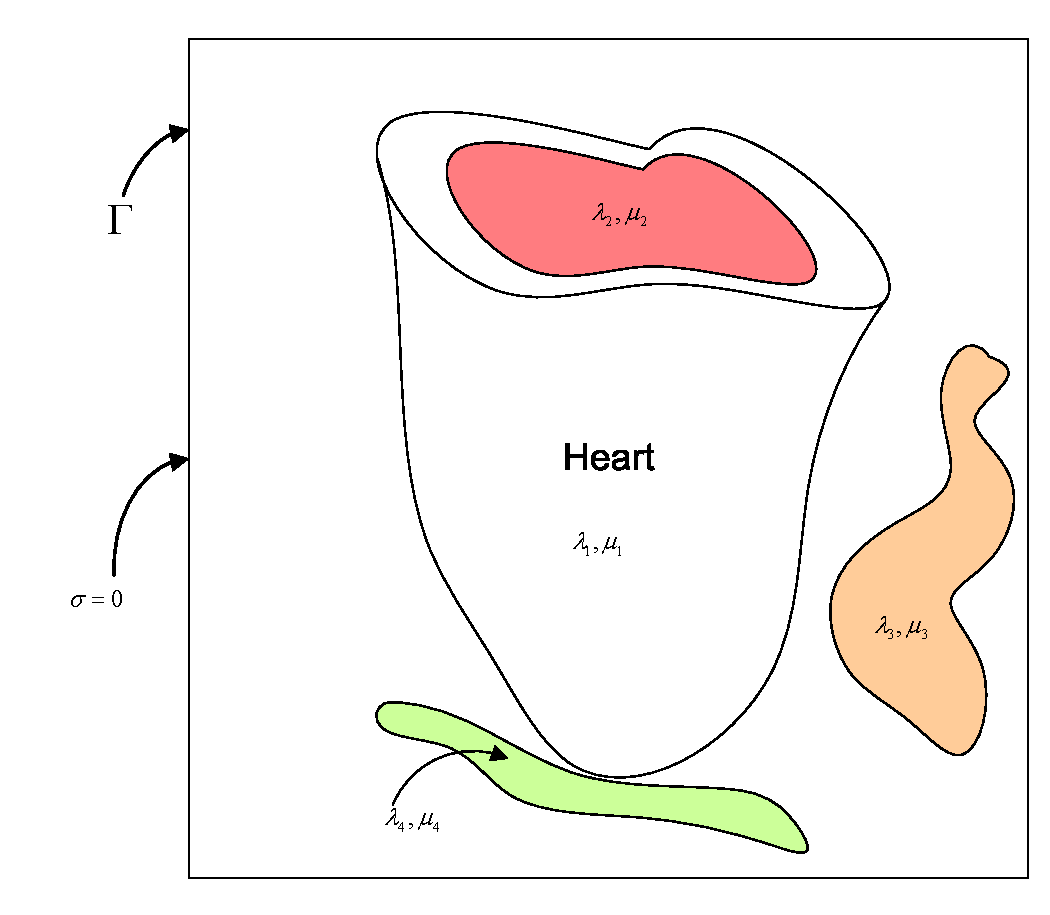
\includegraphics[width=0.5\textwidth]{images/mat_prop}
  \caption{\em \small The material properties and boundary conditions for the cardiac model. We set the stress, $\sigma = 0$, at the boundary $\Gamma$. Different Lam\'{e}  parameters are selected for the myocardium ($\lambda_1, \mu_1$), blood ($\lambda_2, \mu_2)$, the lungs ($\lambda_3, \mu_3)$ and for bone ($\lambda_4, \mu_4)$ }
 \label{matprop}
\end{figure}	

We consider the input data as defined by the MR/DTI image to define the regular domain $\Omega$. The boundary conditions are exactly prescribed on the six faces of the cuboid, $\Gamma$, are simply set to have zero stress, i.e., $\sigma = 0$. One important issue is the accurate integration of the elements that overlap in the inhomogeneity transition. For simplicity we have used voxelized material	properties even in the case of exact geometry information. Within the regular domain $\Omega$, different material properties are assigned based on the tissue type. We currently consider the myocardium ($\lambda_1, \mu_1$), blood ($\lambda_2, \mu_2$), the lungs ($\lambda_3, \mu_3$) and bone ($\lambda_4, \mu_4$). These are shown in Figure \ref{matprop}.

%(This is easy to modify with small computational costs).  The second case, ( case (c) in figure \ref{fig:alg}) corresponds to {\bf Dirichlet	conditions} which we approximate by a constrained optimization approach in which the Dirichlet conditions are imposed through either Lagrange multipliers, or a simpler penalty formulation	\cite{babuska-73}. The latter corresponds to having a very stiff material surrounding the target domain. The nonzero case is treated	by linearity: we construct a smooth function $w(x)$ such that $w(x) = g(x)$ on $\gamma$, where $g(x)$ are the specified boundary conditions. We represent the solution of $L u(x) = f(x)$ as $u = w	+ v$, and we solve for $L v(x) = f - L w(x)$ with homogeneous Dirichlet conditions ($L$ is the linear elasticity operator); $w(x)$ is constructed using a triangulation, or a level-set representation of the boundary.  {\bf Neumann conditions} are imposed using a soft material ( case (d) in fig. \ref{fig:alg}). If $\sigma$ is the imposed stress, the weak form of a Neumann problem (for the Laplacian operator for simplicity) is given by $\int_{\omega}\nabla u\cdot\nabla v=\int_{\gamma}\sigma v$, for all $v$. Using the characteristic function $\chi_{\omega}$ (its value is one inside $\omega$ and zero outside), the weak form becomes $\int_{\Omega}\chi_{\omega}\nabla u\cdot \nabla v = \int_{\gamma}\sigma v$. We can approximate $\chi_{\omega}$ by using a soft material outside $\omega$.

%More complex boundary conditions are not as straightforward. The case in which a Dirichlet condition is specified in the normal direction, and a Neumann condition on the tangent plane can be approximated by anisotropic fictitious materials which are stiff in the normal direction and soft in the tangential direction. Mixed conditions in which part of the boundary is Neumann and part is Dirichlet require more complicated material selection for $\Omega\backslash\omega$. The convergence rates are suboptimal for the jumps in the material properties, whereas the boundary conditions are satisfied only approximately---for the Neumann and Dirichlet cases.

\subsubsection{Multigrid acceleration.} Multigrid methodologies have revolutionized scientific computation, especially for elliptic partial differential equations. Multigrid solvers consist of three main components: the smoother that reduces the algebraic residual at each level, and the restriction and prolongation operators for intergrid transfers \cite{brandt-77}. Typical smoothers are stationary iterative solvers, e.g. Gauss-Seidel. The multigrid method works very well for constant coefficient PDEs, but slows down for strongly variable coefficient problems.  In \cite{alcouffe-brandt-etal-81} a multigrid method for high-contrast materials is presented but is quite restrictive: material property jumps have to align with the grid. Algebraic multigrid is another alternative, but it requires an assembled matrix; this is costly and incompatible with our goals. Here we use a different approach. We are not using the multigrid algorithm to solve, but rather {\em to precondition} a Krylov method. Furthermore the smoothers within the multigrid iteration consist of a number of preconditioned Krylov iterations. We are using a Conjugate Gradient solver both to drive the overall residual, and as a smoother at each level. For high-contrast materials it is important to precondition the smoothers too; we have found that a simple damped Jacobi method suffices to obtain good algorithmic scalability. We use classical full-weighting and linear interpolation intergrid transfer operators. Extensive numerical tests have demonstrated robustness on high contrast inhomogeneities.  Our code is developed on top of PETSc~\cite{petsc-home-page}, a scientific computing library from Argonne National Laboratory.	

\section{Diffusion Tensor Imaging}

Diffusion tensor Imaging (DTI) is a technique to measure the anisotropic diffusion properties of biological tissues within the sample. This allows us to noninvasively infer the structure of the underlying tissue. Diffusion properties allow the classification of different types of tissues and can be used for tissue segmentation and detecting tissue orientations. The principal eigenvector of the diffusion tensor is known to align with fiber tracts in the brain \cite{pierpaoli96} and in the heart \cite{scollan98}. Heart fibers reconstructed from cardiac DTI are shown in Figure \ref{fibers-dti}.

Diffusion tensors describe the diffusion properties of water molecules. In tissues diffusion properties are dictated by the cell structure of the tissue. Since cell membranes are selectively permeable, water molecules can move easily within a cell, but their diffusion across the membrane is limited. Thus diffusion properties of the tissue reflect the shape and orientation of the cells. For the specific case of elongated cells like the cardiac muscles, the diffusion will be maximum along the primary axis of the muscle, which also happens to be the direction along which maximum strain is developed.

\begin{figure}
\begin{center}
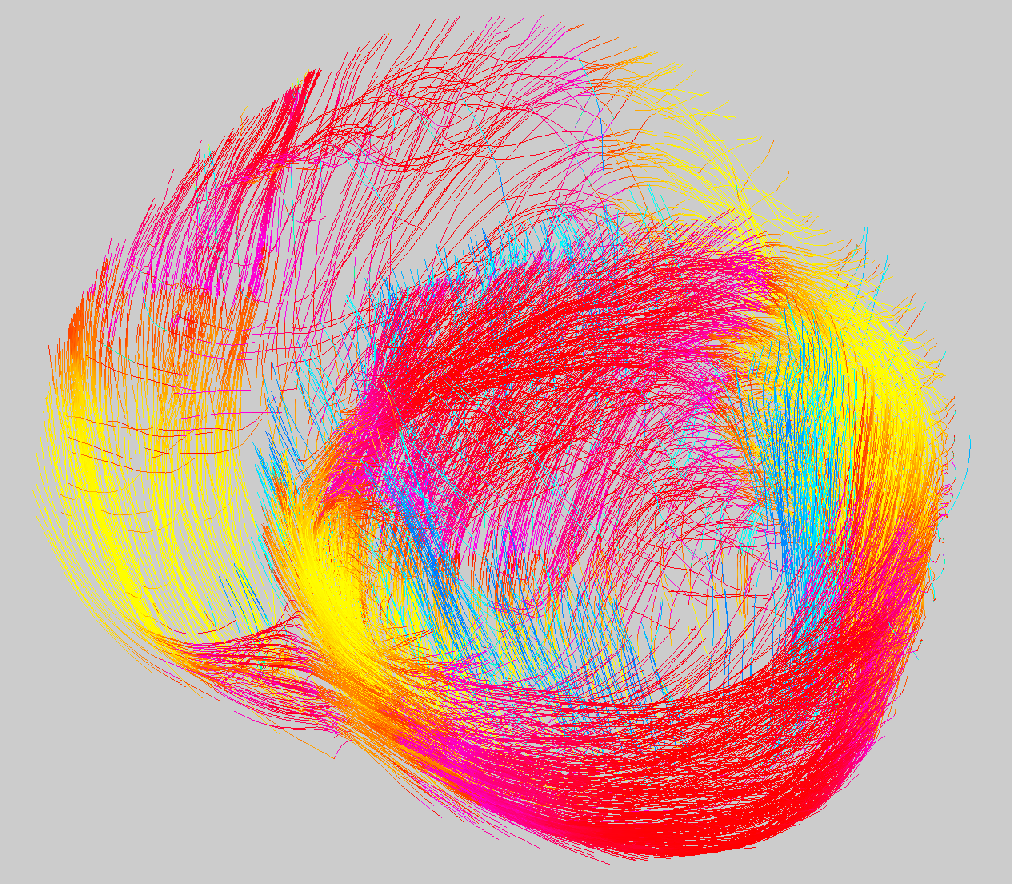
\includegraphics[width=0.4\textwidth]{images/fibers3}
\caption{\em \small Heart fiber orientation in the human heart, obtained from diffusion tensor imaging}
\label{fibers-dti}
\end{center}  
\end{figure} 

Diffusion is measured through a diffusion coefficient, which is represented as a symmetric second order tensor:

\begin{equation}
\label{eq:dt}
{\bf D} = \left( 				
\begin{array}{ccc}
D_{xx} & D_{xy} & D_{xz} \\
D_{yx} & D_{yy} & D_{yz} \\	
D_{zx} & D_{zy} & D_{zz}
\end{array}
          \right)
\end{equation}
The 6 independent values of the tensor elements vary continuously with the spatial location in the tissue.

Eigenvalues $\lambda_i$ and eigenvectors ${\bf e}_i$ of the diffusion tensor (\ref{eq:dt}) can be found
as a solution to the eigenvalue problem:
\[
{\bf De}_i = \lambda_i{\bf e}_i
\]
Since the tensor is symmetric, its eigenvalues are always real numbers, and the eigenvectors are orthogonal and form a basis. Geometrically, a diffusion tensor can be thought of as an ellipsoid with its three axes oriented along these eigenvectors, with the three semiaxis lengths proportional to the square root of the eigenvalues of the tensor.

% Using the ellipsoidal interpretation, one can classify the diffusion properties of a tissue according to the shape of the ellipsoids, with extended ellipsoids corresponding to regions with strong linear diffusion (long, thin cells), flat ellipsoids to planar diffusion, and spherical ellipsoids to regions of isotropic media (such as fluid filled regions like the ventricles). The quantitative classification can be done through the coefficients $c_l$, $c_p$, $c_s$ corresponding to linear, planar and spherical diffusion.
%\begin{eqnarray*}
%c_l &=& \frac{\lambda_1 - \lambda_2}{\lambda_1 + \lambda_2 + \lambda_3} \\
%c_l &=& \frac{2(\lambda_2 - \lambda_3)}{\lambda_1 + \lambda_2 + \lambda_3} \\
%c_l &=& \frac{3\lambda_1}{\lambda_1 + \lambda_2 + \lambda_3}
%\end{eqnarray*}

The heart fibers have strong linear diffusion %($\lambda_1 >> \lambda_2 \approx \lambda_3)$ 
and are oriented along the principal eigenvector, ${\bf e}_1$ \cite{tseng99, scollan98}. Therefore if we need fiber orientations for a specific subject, then computing the principal direction of the diffusion tensor is sufficient. However, {\em in vivo} acquisition of cardiac DTI is not possible using current scanners and acquisition protocols. Consequently, we use an alternate strategy and map the diffusion tensors from a template image onto the subject. The procedure for warping DTIs from a template onto a subject is described in the following section.

\section {Warping Diffusion Tensors from template to subjects}

We have MR images for both the subject and the template. The diffusion tensor data is available only for the template. We use a very high dimensional elastic registration technique \cite{hammer} to estimate the deformation that warps the template to the subject space. We use this deformation field to map the fibers from the template to the subject. It is more complicated to warp tensor fields than it is to warp scalar images. This is because the tensor must be reoriented on each image voxel, in addition to a voxel displacement that is implied by the deformation field. This is achieved by finding the rotational component of the deformation field. We test the effectiveness of the tensor remapping algorithm by comparing the mapped tensors with the ground truth diffusion tensors for 19 canine datasets\footnote{CCBM, Johns Hopkins University}. The method of computing the transformation between the two geometries and the tensor reorientation algorithm are now described.

\subsection{Deformable Image Registration}

Image warping for deformable registration has received a great deal of attention during the past decade \cite{Zitova03}. In the present work we used a very-high-dimensional elastic transformation procedure in 3D volume space, referred to as the hierarchical attribute matching mechanism for elastic registration (HAMMER) method, which is determined from T1-weighted images and applied on the coregistered DT image of the template. This approach uses image attributes to determine point correspondences between an individual image and a template, which resides in the stereotaxic space and is the subject for which we have the diffusion tensors. A hierarchical sequence of piece-wise smooth transformations is then determined, so that the attributes of the warped images are as similar as possible to the attributes of the target. Relatively fewer, more stable attributes are used in the initial stages of this procedure, which helps avoid local minima, a known problem in high-dimensional transformations. The details of this algorithm can be found in \cite{hammer}.


\subsection{Tensor Reorientation}
It is a simple matter to warp a scalar image by a known spatial transformation. The image value from a particular voxel is transferred, via the displacement field of the spatial transformation, to a voxel in the target image. Typically, some sort of interpolation must also be applied. However, a more complex procedure is required to warp tensor fields, especially when the tensor estimates are noisy. We use an approach similar to that proposed by Xu et al \cite{xu03}.

If we know the direction, ${\bf v}$, of the fiber on voxel with coordinates ${\bf x}$, we can readily find the rotated version, ${\bf v}'$, of ${\bf v}$, according to the warping transformation. If ${\bf R}$ is the matrix that rotates ${\bf v}$ to ${\bf v'}$, then ${\bf R}$ should be applied to the respective tensor measurement. However, in practice we do not know ${\bf v}$. In fact, this is precisely what we would like to estimate. We only have a noisy orientation of $v$, which is the principal direction (PD) of the corresponding tensor measurement. One could use that PD in place of ${\bf v}$, as proposed in \cite{alex01}. However, that makes the approach vulnerable to noise, since the PD is only a noisy observation, and could be quite different from the true underlying fiber orientation. 

Assuming that we know the probability distribution function (PDF), $f({\bf v})$, of the fiber direction ${\bf v}$, we can find the rotation matrix, $\tilde{\bf R}$ which minimizes the expected value of $\|{\bf v' -Rv} \|^2$ over all orthonormal matrices ${\bf R}$:

\begin{eqnarray*}
\tilde{\bf R} &=& \mathop{\arg \min}_{\bf R} E\{\|{\bf v' -Rv} \|^2\}\\
&=& \mathop{\arg \min}_{\bf R} \int_{\bf v} pdf({\bf v}) \|{\bf v' -Rv} \|^2 d{\bf v}
\end{eqnarray*}

This problem can be solved by the Procrustean estimation \cite{golub83}, if a number of random samples, ${\bf v}$, are drawn from the PDF, and their respective rotated versions, ${\bf v'}$, are found by the rotation that the warping field applies to ${\bf v}$. If we arrange these vectors ${\bf v'}$ and ${\bf v}$ to form the columns of the matrices ${\bf A}$ and ${\bf B}$, respectively, then $\tilde{\bf R}$ is found by minimizing:
\[
	\left\|{\bf A} - {\bf R}\cdot{\bf B}\right\|_2^2 = \left\|{\bf A}\right\|_2^2 + \left\|{\bf B}\right\|_2^2 + 2\sum_i\sigma_i({\bf A}\cdot{\bf B}^T)
\]

where $\sigma_i(\bM)$ are the singular values of matrix ${\bf M}$. $\tilde{\bf R}$ can be determined via a singular value decomposition of ${\bf A \cdot B}$.

\begin{eqnarray*}
{\bf A}\cdot{\bf B}^T &=& {\bf V}\cdot\Sigma\cdot {\bf W}^T \\
\tilde{\bf R} &=& {\bf V}\cdot{\bf W}^T 
\end{eqnarray*}

More details on the algorithm and the estimation of the PDF can be found in \cite{xu03}.

\section{Results and Validation}

We used canine DTI datasets obtained from Center for Cardiovascular Bioinformatics and Modeling, Johns Hopkins University and acquired at the National Institue of Health, to validate the effectiveness of our diffusion tensor remapping algorithm. A total of $19$ canine subjects were scanned, of which $12$ subjects were normal, and $7$ had cardiac failure. The scans were performed {\em in vitro} after the hearts were harvested. Each heart was placed in an acrylic container filled with Fomblin, a perfluoropolyether (Ausimon, Thorofare, NJ). Fomblin has a low dielectric effect and minimal MR signal, thereby increasing contrast and eliminating unwanted susceptibility artifacts near the boundaries of the heart.  The long axis of the hearts was aligned with the $z$ axis of the scanner.  Images were acquired with a 4-element knee phased array coil on a 1.5 T GE CV/I MRI Scanner (GE, Medical System, Wausheka, WI) using an enhanced gradient system with 40 mT/m maximum gradient amplitude and a 150 T/m/s slew rate.

Since only the long axis of the heart was aligned with the $z$ axis of the scanner, we first need to correct for rotation about the $z$ axis. We picked one of the normal canine hearts as the template, and performed affine registration to warp the remaining subjects onto the template space. The diffusion tensors for these subjects were also rotated by the rotational component of the affine transform. We then perform the elastic registration using HAMMER to estimate the transformation that maps the template to the subject space. This transformation is then used to warp and reorient the diffusion tensors of template onto the subject. The quality of the mapping is measured by computing the angle between the principal direction of the mapped tensor and the principal direction of the ground truth obtained from the subject's DTI. This is shown in Figure \ref{fig:dot}.

The error in the fiber orientations is further demonstrated on one slice in Figure \ref{fig:pd_both}, by comparing the original fibers (in red) and the mapped fibers (in blue). Our method was able to successfully map the fibers for healthy as well as for failing canine hearts. The percentage of voxels where the error in the principal directions is less than $10^\circ$ is shown in Figure \ref{fig:graph}. We evaluate an error of less than $10^\circ$ since it is close to the average error obtained from DTI imaging \cite{scollan98} and histological measurements\cite{streeter73}. We also compare this with the error by using a synthetic model to estimate fiber orientations. The synthetic fiber orientations were produced by varying the elevation angle between the short axis plane and the fiber between $+90^\circ$ and $-90^\circ$ from the endocardium to the epicardium. Similar synthetic models have been used in \cite{sachse04, sermesant04}.

\begin{figure}
\begin{center}
\framebox{
%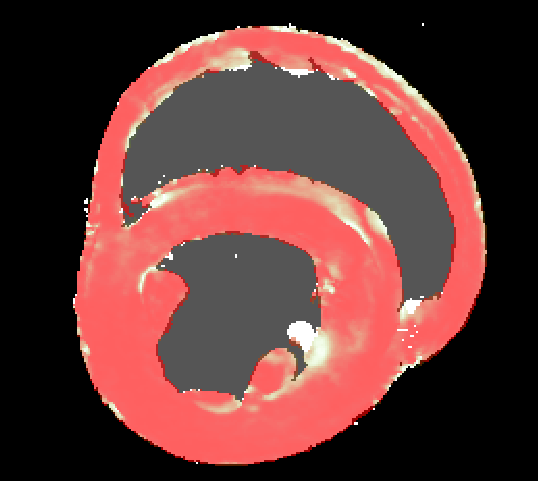
\includegraphics[width=0.4\textwidth]{images/dot_prod} 
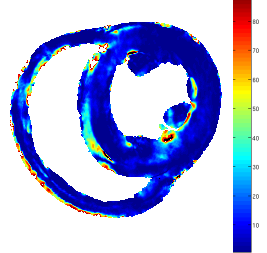
\includegraphics[width=0.4\textwidth]{images/dot}}
\caption{\em \small The angle between the mapped principal direction with the actual principal direction, in degrees. The image is overlaid on a segmentation of the heart based on the fractional anisotropy } 
\label{fig:dot}
\end{center}  
\end{figure} 

%Also in order to verify whether the fiber orientations are sufficiently close for fiber tracking purposes, we created a checkerboard DTI using the original and mapped DTIs.  We performed fiber tracking on this checkerboard DTI and the resulting fibers are shown in Figure Y, alongside the fibers obtained from only the original DTI. 
%The method was able to successfully map the fibers for healthy as well as for failing canine hearts. The percentage of voxels where the error the principal directions is less than $10^\circ$ is shown in Figure \ref{fig:graph}. 

%The plot also shows the error introduced in the same heart where a synthetic model was used to estimate the fiber orientations. The synthetic fiber orientations were produced by varying the elevation angle between the short axis plane and the fiber between $+90^\circ$ and $-90^\circ$ from the endocardium to the epicardium. Similar synthetic models have been used in CITE metaxas, Semersant, sachse.

The method was able to map the fibers accurately for both healthy as well as for failing hearts that had left bundle branch blocks. Although, the percentage of voxels having an error of less than $10^\circ$ was lower in the failing hearts as compared to the healthy ones, we observe that most of these errors are in the vicinity of the block as expected, and the fiber orientations away from the bundle branch block were similar to that observed in healthy patients. Therefore, our method should perform better for other pathologies like ventricular hypertropy and infarction, since it has been shown that the muscle fiber orientations are not affected significantly by hypertrophy and myocardial infarction\cite{walker05}. 

\begin{figure}
\begin{center}
%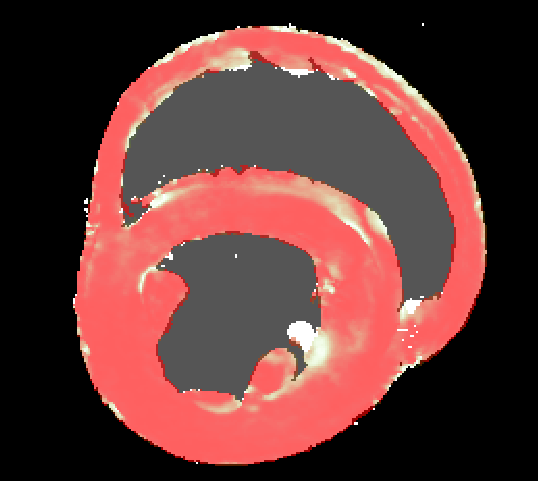
\includegraphics[width=0.4\textwidth]{images/dot_prod} 
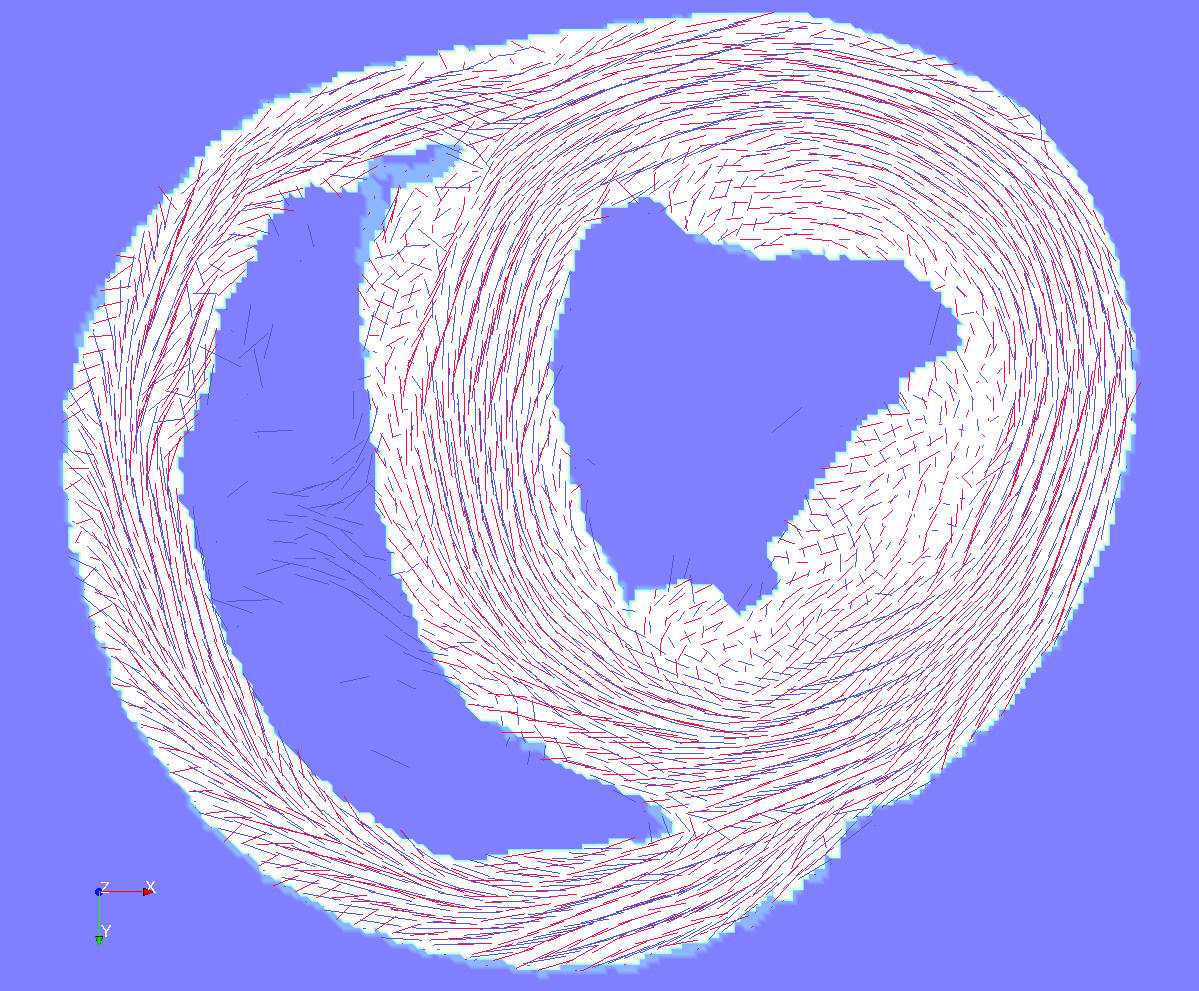
\includegraphics[width=0.5\textwidth]{images/pd_mapped_dti_2} 
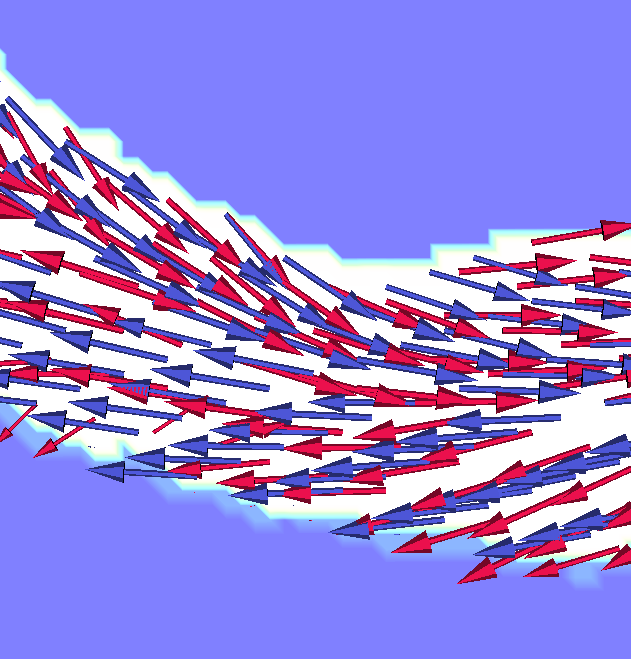
\includegraphics[width=0.395\textwidth]{images/pd_mapped_dti_3} 
\caption{\em \small The principal directions of the original DT are shown in blue. The mapped principal directions are shown in red. The glyphs are overlaid on a segmentation of the heart based on the fractional anisotropy of the mapped DT}
\label{fig:pd_both}
\end{center}  
\end{figure} 

\begin{figure}
\begin{center}
%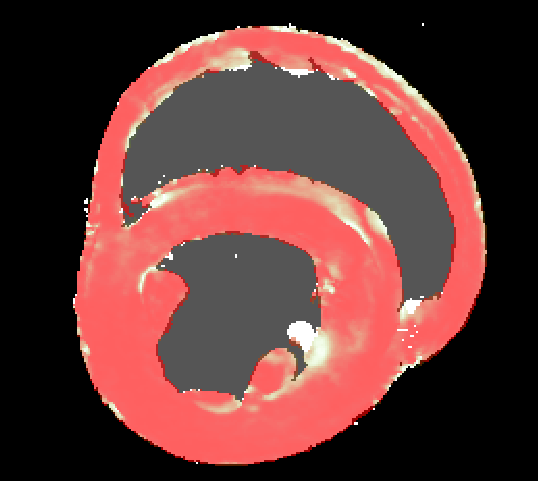
\includegraphics[width=0.4\textwidth]{images/dot_prod} 
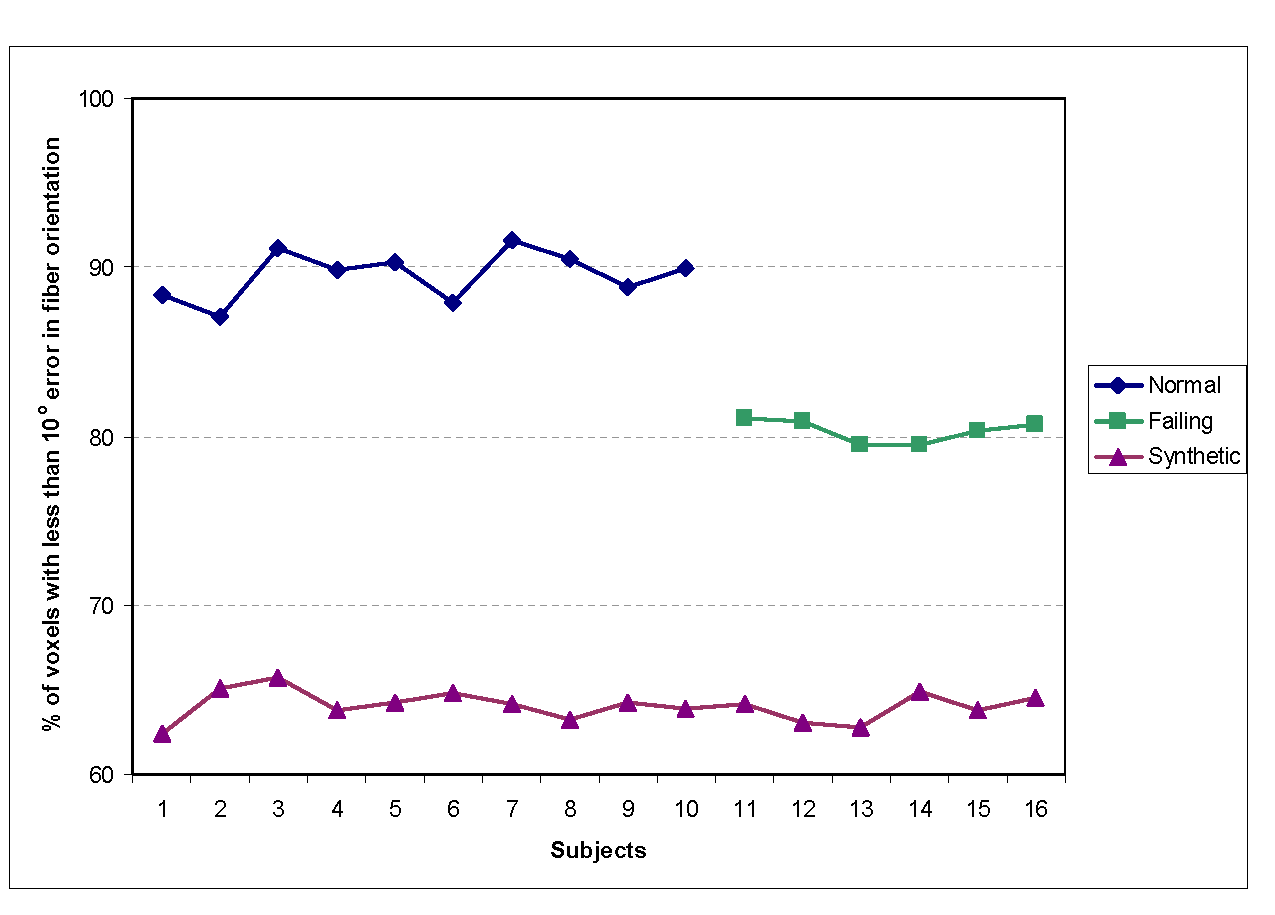
\includegraphics[width=0.8\textwidth]{images/graph} 
\caption{\em \small The percentage of voxels having less than $10^\circ$ error in the principal directions after mapping }
\label{fig:graph}
\end{center}  
\end{figure} 
